% KARMA - IEEE Conference Paper
% Compile with: pdflatex research_paper_v2.tex
\documentclass[conference]{IEEEtran}

\usepackage{cite}
\usepackage{amsmath,amssymb,amsfonts}
\usepackage{algorithmic}
\usepackage{graphicx}
\usepackage{textcomp}
\usepackage{xcolor}
\usepackage{booktabs}
\usepackage{multirow}
\usepackage{hyperref}
\usepackage{listings}
\usepackage{tikz}
\usetikzlibrary{shapes.geometric, arrows, positioning, fit, calc}

% Listing style for code snippets
\lstset{
  basicstyle=\ttfamily\footnotesize,
  breaklines=true,
  frame=single,
  numbers=left,
  numberstyle=\tiny,
  tabsize=2
}

% TikZ styles for architecture diagrams
\tikzstyle{block} = [rectangle, draw, fill=blue!10, text width=5.5em, text centered, rounded corners, minimum height=2.5em, font=\footnotesize]
\tikzstyle{store} = [cylinder, draw, fill=green!10, shape border rotate=90, aspect=0.25, minimum height=2em, minimum width=4em, font=\footnotesize]
\tikzstyle{data} = [rectangle, draw, fill=orange!10, text width=4.5em, text centered, minimum height=2em, font=\footnotesize]
\tikzstyle{arrow} = [thick,->,>=stealth]
\tikzstyle{biarrow} = [thick,<->,>=stealth]

\begin{document}

\title{KARMA: A Multi-Agent Framework with Active Knowledge Base Learning for Autonomous Financial Investment Decisions}

\author{\IEEEauthorblockN{Lakshya Sharma}
\IEEEauthorblockA{Department of Computer Science\\
Email: lakshya@example.edu}}

\maketitle

\begin{abstract}
Large Language Models (LLMs) have demonstrated considerable promise in financial text analysis, yet their deployment in autonomous investment decision-making remains constrained by three fundamental limitations: the absence of temporal memory across trading sessions, reliance on static knowledge that cannot adapt to evolving market conditions, and opaque reasoning that lacks explainability. While Retrieval-Augmented Generation (RAG) has emerged as a solution for grounding LLM outputs in external knowledge, existing implementations in finance remain predominantly \textit{passive}---retrieving static documents without learning from their own performance. This paper introduces \textbf{KARMA}, a novel multi-agent framework featuring an \textit{Active Knowledge Base (KB) Agent} that transforms RAG from a read-only retrieval mechanism into a read-write learning system. The KB Agent operates across three phases of the decision lifecycle: \textbf{pre-query} (retrieving historical context and lessons learned before analysis), \textbf{post-learn} (storing structured decision records after trading), and \textbf{outcome reflection} (generating lessons from realized returns to improve future decisions). Built on LangGraph with a 12-node agent pipeline and ChromaDB with three specialized vector stores, KARMA orchestrates four domain analysts, bull/bear researchers, a risk manager, and a trader agent---all grounded by an evolving institutional memory. Experimental evaluation on a portfolio of five major equities demonstrates that the system produces contextually informed, explainable investment recommendations that improve over successive trading sessions through its self-reinforcing feedback loop.
\end{abstract}

\begin{IEEEkeywords}
Agentic RAG, Multi-Agent Systems, Knowledge Base Agent, Retrieval-Augmented Generation, LangGraph, Financial Decision-Making, Explainability, Active Learning
\end{IEEEkeywords}

% ============================================================
\section{Introduction}
% ============================================================

The financial domain presents unique challenges for artificial intelligence, characterized by high volatility, data heterogeneity spanning numerical time-series and unstructured text, and the critical need for transparent, explainable reasoning~\cite{minaee2024llm}. Large Language Models (LLMs) such as GPT-4~\cite{openai2023gpt4} have shown remarkable capability in processing financial text, including earnings reports, news articles, and social media sentiment. However, when applied to autonomous trading, they exhibit three critical limitations:

\begin{enumerate}
\item \textbf{Memory Amnesia}: Each analysis is treated as an isolated event. The system fails to recall prior analyses of the same stock under similar conditions.
\item \textbf{Static Knowledge}: While standard RAG~\cite{lewis2020rag} addresses the knowledge cutoff by retrieving external documents, these implementations are read-only---the system retrieves what exists but does not synthesize new knowledge from its own experience.
\item \textbf{Lack of Reflection}: LLMs do not natively verify whether past predictions were correct, precluding outcome-based learning.
\end{enumerate}

Recent work in multi-agent financial systems, particularly TradingAgents~\cite{tradingagents2024}, has demonstrated the value of role-specialized agents communicating through structured debate. However, these frameworks lack a centralized, evolving memory---agents debate from scratch each session.

Concurrently, the emerging paradigm of Agentic RAG~\cite{singh2025agenticrag} has been identified as a transformative advancement, embedding autonomous agents into the RAG pipeline. Singh et al.~\cite{singh2025agenticrag} provide a comprehensive taxonomy of Agentic RAG architectures---single-agent routers, multi-agent systems, hierarchical architectures, corrective RAG, and adaptive RAG---but note that few implementations close the feedback loop between decisions and outcomes.

\textbf{KARMA bridges this gap.} We propose a framework in which the RAG system is elevated from a passive retrieval tool to an active, learning participant. The core novelty is the \textbf{Knowledge Base (KB) Agent}, a dedicated entity that orchestrates the flow of experience: querying historical context \textit{before} analysis, storing structured decisions \textit{after} trading, and generating reflective lessons when actual returns are realized.

\subsection{Research Objectives}

\begin{enumerate}
\item \textbf{Design and implement an Active KB Agent} that transforms RAG from passive retrieval to active, bidirectional knowledge management within a multi-agent financial analysis pipeline.
\item \textbf{Develop a three-store Multi-RAG architecture} with specialized vector collections for market insights, trade history, and lessons learned.
\item \textbf{Evaluate the framework's capacity} for producing explainable, context-aware investment decisions that improve through outcome-based feedback loops.
\end{enumerate}

% ============================================================
\section{Literature Review}
% ============================================================

\subsection{Retrieval-Augmented Generation}

Retrieval-Augmented Generation (RAG), introduced by Lewis et al.~\cite{lewis2020rag}, combines parametric memory (LLM weights) with non-parametric memory (external knowledge bases). The paradigm has evolved through several stages~\cite{gao2024ragsurvey}: \textit{Na\"ive RAG} relies on keyword-based retrieval; \textit{Advanced RAG} introduces dense passage retrieval (DPR) and neural re-ranking; \textit{Modular RAG} decomposes the pipeline into reusable components; and \textit{Graph RAG}~\cite{peng2024graphrag} leverages structured relationships for multi-hop reasoning.

In finance, RAG has been applied to retrieve SEC filings and news articles. FinGPT~\cite{yang2023fingpt} and BloombergGPT~\cite{wu2023bloomberggpt} represent notable efforts, though their RAG components remain read-only.

\subsection{Agentic RAG}

The convergence of RAG and agentic intelligence has produced Agentic RAG~\cite{singh2025agenticrag}, introducing autonomous agents capable of dynamic decision-making and iterative refinement. Singh et al.~\cite{singh2025agenticrag} identify four foundational agentic patterns: \textit{Reflection}~\cite{madaan2023selfrefine}, \textit{Planning}, \textit{Tool Use}, and \textit{Multi-Agent Collaboration}~\cite{singh2024agentic}.

Key architectural variants include Corrective RAG~\cite{yan2024crag} with self-correction mechanisms and Adaptive RAG~\cite{jeong2024adaptive} that dynamically adjusts retrieval strategy. Our work extends Multi-Agent Agentic RAG with a dedicated memory management agent implementing all four agentic patterns.

\subsection{Multi-Agent Systems in Finance}

TradingAgents~\cite{tradingagents2024} proposes a multi-agent framework simulating a trading firm with fundamental, technical, and sentiment analysts, researchers engaging in bull/bear debate, a risk manager, and a fund manager. AutoGen~\cite{wu2023autogen} and CrewAI~\cite{crewai2025} provide general multi-agent frameworks. However, all share a common limitation: the absence of persistent, evolving memory across trading sessions.

\subsection{Cognitive Architectures and Reflection}

Our architecture draws from cognitive science, specifically hippocampal memory consolidation~\cite{zhang2024memory}. Park et al.~\cite{park2023generative} demonstrated generative agents with memory streams and reflection. Shinn et al.~\cite{shinn2023reflexion} introduced Reflexion for verbal reinforcement learning. We apply analogous mechanisms to financial trading, introducing outcome-based reinforcement from realized returns.

% ============================================================
\section{Methodology}
% ============================================================

\subsection{System Architecture Overview}

KARMA is built on a modular multi-agent architecture orchestrated via LangGraph~\cite{langgraph2025}. The system comprises: (1)~a multi-source data ingestion pipeline, (2)~a team of 10 specialized LLM agents organized in a 12-node pipeline, (3)~a three-store Multi-RAG knowledge system managed by ChromaDB~\cite{chromadb2025}, and (4)~an explainability and outcome learning module. Fig.~\ref{fig:architecture} illustrates the overall architecture.

\begin{figure}[htbp]
\centering
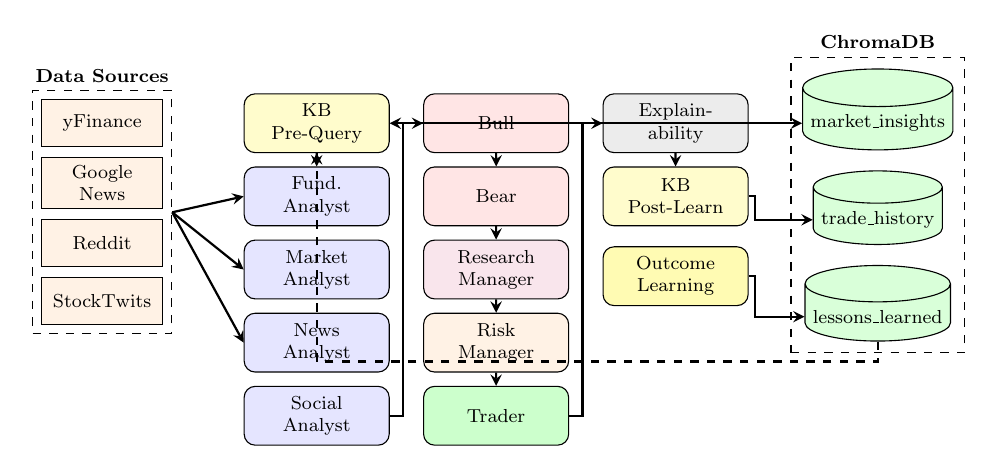
\begin{tikzpicture}[node distance=0.6cm and 0.4cm, scale=0.85, every node/.style={transform shape}]

% Data sources
\node[data] (yf) {yFinance};
\node[data, below=0.15cm of yf] (gn) {Google\\News};
\node[data, below=0.15cm of gn] (rd) {Reddit};
\node[data, below=0.15cm of rd] (st) {StockTwits};

% Data box
\node[draw, dashed, fit=(yf)(gn)(rd)(st), inner sep=3pt, label=above:{\footnotesize\textbf{Data Sources}}] (databox) {};

% Agent pipeline
\node[block, right=1.2cm of yf, fill=yellow!20] (kb1) {KB\\Pre-Query};
\node[block, below=0.2cm of kb1, fill=blue!10] (fa) {Fund.\\Analyst};
\node[block, below=0.2cm of fa, fill=blue!10] (ma) {Market\\Analyst};
\node[block, below=0.2cm of ma, fill=blue!10] (na) {News\\Analyst};
\node[block, below=0.2cm of na, fill=blue!10] (sa) {Social\\Analyst};

\node[block, right=0.5cm of kb1, fill=red!10] (bull) {Bull};
\node[block, below=0.2cm of bull, fill=red!10] (bear) {Bear};
\node[block, below=0.2cm of bear, fill=purple!10] (rm) {Research\\Manager};
\node[block, below=0.2cm of rm, fill=orange!10] (risk) {Risk\\Manager};
\node[block, below=0.2cm of risk, fill=green!20] (trader) {Trader};

\node[block, right=0.5cm of bull, fill=gray!15] (expl) {Explain-\\ability};
\node[block, below=0.2cm of expl, fill=yellow!20] (kb2) {KB\\Post-Learn};

% Knowledge stores
\node[store, right=0.8cm of expl, fill=green!15] (mi) {market\_\\insights};
\node[store, below=0.3cm of mi, fill=green!15] (th) {trade\_\\history};
\node[store, below=0.3cm of th, fill=green!15] (ll) {lessons\_\\learned};

\node[draw, dashed, fit=(mi)(th)(ll), inner sep=4pt, label=above:{\footnotesize\textbf{ChromaDB}}] (kbbox) {};

% Arrows: data → agents
\draw[arrow] (databox.east) -- (fa.west);
\draw[arrow] (databox.east) -- (ma.west);
\draw[arrow] (databox.east) -- (na.west);

% Pipeline flow
\draw[arrow] (kb1) -- (fa);
\draw[arrow] (sa.east) -- ++(0.2,0) |- (bull.west);
\draw[arrow] (bull) -- (bear);
\draw[arrow] (bear) -- (rm);
\draw[arrow] (rm) -- (risk);
\draw[arrow] (risk) -- (trader);
\draw[arrow] (trader.east) -- ++(0.2,0) |- (expl.west);
\draw[arrow] (expl) -- (kb2);

% KB ↔ stores
\draw[biarrow] (kb1.east) -- ++(0.1,0) |- (mi.west);
\draw[arrow] (kb2.east) -- ++(0.1,0) |- (th.west);

% Outcome learning
\node[block, below=0.3cm of kb2, fill=yellow!30] (ol) {Outcome\\Learning};
\draw[arrow] (ol.east) -- ++(0.1,0) |- (ll.west);
\draw[arrow, dashed] (ll.south) -- ++(0,-0.3) -| (kb1.south);

\end{tikzpicture}
\caption{KARMA system architecture. The 12-node LangGraph pipeline features bidirectional RAG integration via the KB Agent. Dashed arrow shows the feedback loop: lessons learned from outcomes inform future pre-queries.}
\label{fig:architecture}
\end{figure}

\subsection{The Active Knowledge Base Agent}

The \textbf{KB Agent} is the core novelty. Unlike passive RAG implementations, the KB Agent actively participates in three distinct phases:

\textbf{Phase 1---Pre-Analysis Query (Recall).} Before any analyst begins, the KB Agent queries all three ChromaDB collections using the target ticker. It synthesizes a \texttt{Historical Context} report containing:
\begin{itemize}
\item \textit{Market Insights}: Historical patterns and observations.
\item \textit{Trade History}: Prior decisions with dates and confidence levels.
\item \textit{Lessons Learned}: Outcome-based lessons (e.g., ``FAILED BUY on NVDA: ignored overbought RSI'').
\end{itemize}
This context is injected into every analyst's prompt.

\textbf{Phase 2---Post-Decision Storage (Consolidation).} After the Trader agent produces a decision, the KB Agent captures the full state---all analyst reports, the bull/bear debate, risk assessment, and reasoning---storing it as a structured record in \texttt{trade\_history} and key insights in \texttt{market\_insights}.

\textbf{Phase 3---Outcome Reflection (Learning).} When actual returns are realized, the system compares the decision against the return. An LLM generates a reflective lesson:
\begin{itemize}
\item \textit{Success}: ``BUY validated (+5.2\%). Social sentiment correctly predicted earnings surprise.''
\item \textit{Failure}: ``BUY was WRONG ($-$3.1\%). Ignored overbought RSI divergence.''
\end{itemize}
This lesson is stored in \texttt{lessons\_learned} and retrieved during future Pre-Analysis Queries, closing the feedback loop.

\subsection{Multi-RAG Knowledge Stores}

The system maintains three semantically distinct ChromaDB collections (Table~\ref{tab:stores}):

\begin{table}[htbp]
\caption{Multi-RAG Knowledge Store Architecture}
\label{tab:stores}
\centering
\begin{tabular}{@{}lll@{}}
\toprule
\textbf{Store} & \textbf{Purpose} & \textbf{Write Trigger} \\
\midrule
\texttt{market\_insights} & Market observations & Phase 2 \\
\texttt{trade\_history} & Decision log & Phase 2 \\
\texttt{lessons\_learned} & Outcome-derived principles & Phase 3 \\
\bottomrule
\end{tabular}
\end{table}

All stores use OpenAI \texttt{text-embedding-3-small} embeddings. Documents are tagged with metadata including ticker, date, decision type, and outcome correctness.

\subsection{Agent Pipeline}

The 12-node LangGraph \texttt{StateGraph} processes each analysis through the following pipeline:

\begin{enumerate}
\item \textbf{KB Pre-Query}: Retrieves historical context from all three stores.
\item \textbf{Fundamentals Analyst}: Analyzes balance sheet, income, cash flow, and ratios using yFinance data.
\item \textbf{Market Analyst}: Evaluates price action, technicals (MACD, RSI, MAs), support/resistance.
\item \textbf{News Analyst}: Reads 50--100 raw Google News RSS articles; performs independent impact assessment.
\item \textbf{Social Media Analyst}: Analyzes raw Reddit/StockTwits posts with independent sentiment classification.
\item \textbf{Bull Researcher}: Synthesizes positives into the strongest BUY case.
\item \textbf{Bear Researcher}: Synthesizes negatives into the strongest case against BUY.
\item \textbf{Research Manager} (GPT-4o): Weighs bull/bear debate and recommends a direction.
\item \textbf{Risk Manager}: Assesses risk factors, position sizing, stop-loss levels.
\item \textbf{Trader} (GPT-4o): Makes final BUY/HOLD/SELL decision with confidence score.
\item \textbf{Explainability}: Generates comprehensive human-readable report.
\item \textbf{KB Post-Learn}: Stores decision and insights in RAG stores.
\end{enumerate}

Two model tiers are used: \texttt{gpt-4o-mini} for analysts (cost-efficient) and \texttt{gpt-4o} for the Research Manager and Trader (complex reasoning). The system is model-agnostic, supporting OpenAI, Gemini, and Ollama through a centralized configuration hub.

\subsection{Data Ingestion Pipeline}

The \texttt{DataLoader} implements TTL-based JSON caching with configurable fallback chains (Table~\ref{tab:data}). All sources return raw text without pre-computed sentiment, ensuring analysts perform independent analysis.

\begin{table}[htbp]
\caption{Data Source Configuration}
\label{tab:data}
\centering
\begin{tabular}{@{}llll@{}}
\toprule
\textbf{Type} & \textbf{Primary} & \textbf{Fallback} & \textbf{TTL} \\
\midrule
Fundamentals & yFinance & Alpha Vantage & 7 days \\
Market & yFinance & --- & 1 day \\
News & Google RSS & Alpha Vantage & 6 hours \\
Social & Reddit API & StockTwits & 6 hours \\
\bottomrule
\end{tabular}
\end{table}

% ============================================================
\section{Experiments and Results}
% ============================================================

\subsection{Experimental Setup}

We evaluated KARMA using logged runs stored in \texttt{storage/results/\_eval\_sessions.json} and \texttt{storage/results/\_outcomes.json}. The system used GPT-4o (deep reasoning) and GPT-4o-mini (analysts), with ChromaDB and OpenAI \texttt{text-embedding-3-small} embeddings.

The evaluation used a rolling protocol across four session groups between March~3 and March~27, 2026. Most runs analyzed AAPL, GOOGL, and AMZN under two portfolio contexts: \texttt{balanced\_tech} (concentrated existing holdings) and \texttt{fresh\_entry} (no initial holdings). Reported metrics include only entries with available T+1 outcomes (\texttt{was\_correct} not null), yielding 16 checked decisions.

\subsection{Pipeline Execution Analysis}

Each execution traverses all 12 nodes. Table~\ref{tab:pipeline} shows a representative AAPL analysis:

\begin{table}[htbp]
\caption{Agent Pipeline Execution: AAPL (2026-02-07)}
\label{tab:pipeline}
\centering
\footnotesize
\begin{tabular}{@{}clll@{}}
\toprule
\textbf{\#} & \textbf{Agent} & \textbf{Model} & \textbf{Key Output} \\
\midrule
1 & KB Pre-Query & --- & Context from 3 stores \\
2 & Fundamentals & mini & EPS \$7.89, D/E 102.63 \\
3 & Market & mini & +7.37\% 30d, BULLISH \\
4 & News & mini & 59 articles, HIGH impact \\
5 & Social & mini & 1 bullish, 1 bear, 1 neutral \\
6 & Bull & mini & Strong margins, momentum \\
7 & Bear & mini & High D/E, low liquidity \\
8 & Research Mgr & 4o & Mixed signals, moderate \\
9 & Risk Mgr & mini & MEDIUM risk \\
10 & Trader & 4o & \textbf{HOLD} @ 0.75 conf. \\
11 & Explainability & --- & Full report generated \\
12 & KB Post-Learn & --- & Decision stored \\
\bottomrule
\end{tabular}
\end{table}

\subsection{Rolling Evaluation Results}

Table~\ref{tab:aggregate} summarizes checked outcomes from logged sessions.

\begin{table}[htbp]
\caption{Aggregate Evaluation Metrics (Checked T+1 Outcomes)}
\label{tab:aggregate}
\centering
\begin{tabular}{@{}lr@{}}
\toprule
\textbf{Metric} & \textbf{Value} \\
\midrule
Decisions checked (T+1) & 16 \\
Correct decisions & 14 \\
Accuracy & \textbf{87.5\%} \\
Mean T+1 return (all checked) & $-$0.30\% \\
Mean T+1 return (HOLD) & $-$0.13\% \\
Mean T+1 return (BUY) & $-$1.04\% \\
HOLD / BUY / SELL ratio & 81.3\% / 18.7\% / 0\% \\
\bottomrule
\end{tabular}
\end{table}

\begin{table}[htbp]
\caption{Per-Session Checked Outcome Snapshot}
\label{tab:sessionbreakdown}
\centering
\footnotesize
\begin{tabular}{@{}lcccc@{}}
\toprule
\textbf{Session Slice} & \textbf{Checked} & \textbf{Correct} & \textbf{Accuracy} & \textbf{Mix} \\
\midrule
Round 1 Day 1 (balanced\_tech) & 3 & 3 & 100\% & 3 HOLD \\
Round 2 Days 1,2,4 (balanced\_tech) & 9 & 9 & 100\% & 9 HOLD \\
Round 3 Day 1 (fresh\_entry, partial) & 1 & 1 & 100\% & 1 BUY \\
Round 4 Day 1 (fresh\_entry) & 3 & 1 & 33.3\% & 2 BUY, 1 HOLD \\
\bottomrule
\end{tabular}
\end{table}

The key pattern is that HOLD recommendations remained robust in concentrated-risk settings, while BUY decisions were more sensitive to short-term drawdowns in fresh-entry settings.

\subsection{Knowledge Base Evolution}

Table~\ref{tab:kbgrowth} shows how the ChromaDB stores grow over successive sessions, demonstrating the accumulative learning behavior:

\begin{table}[htbp]
\caption{Knowledge Base Growth Across Sessions}
\label{tab:kbgrowth}
\centering
\footnotesize
\begin{tabular}{@{}lcccc@{}}
\toprule
\textbf{Stage} & \textbf{Insights} & \textbf{History} & \textbf{Lessons} & \textbf{Total} \\
\midrule
Initial & 0 & 0 & 0 & 0 \\
After 1 run & 2 & 1 & 0 & 3 \\
After Rd.\ 1 (3 decisions) & 8 & 4 & 0 & 12 \\
+Rd.\ 1 outcomes & 8 & 4 & 3 & 15 \\
After Rd.\ 2 Day 1 & 14 & 7 & 3 & 24 \\
+Rd.\ 2 Day 2 \& outcomes & 20 & 10 & 9 & 39 \\
\bottomrule
\end{tabular}
\end{table}

Round~2 analyses benefited from Round~1's stored context---the KB Pre-Query retrieved prior HOLD decisions and outcomes, reinforcing the system's cautious approach to the concentrated portfolio.

\subsection{Decision Quality Assessment}

\textbf{Case 1---AAPL 2026-02-07 (Empty KB):} The HOLD at 0.75 confidence integrated bullish momentum (+7.37\% monthly return) against concerning fundamentals (D/E 102.63, current ratio 0.974). T+1 return of +1.8\% validated the neutral stance.

\textbf{Case 2---GOOGL 2026-02-17 (Early BUY Signal):} The Research Manager overrode bearish technicals (RSI 32, 5\% decline) for strong fundamentals (\$126.84B cash, 18\% YoY growth, ROE 35.71\%), citing oversold conditions as a buying opportunity.

\textbf{Case 3---Round 4 Day 1 (Fresh-Entry Stress Case):} With no prior holdings, the system produced two BUY signals (AAPL, GOOGL) that were both incorrect at T+1, while HOLD on AMZN was correct. This highlights weaker reliability of directional calls when concentration constraints are absent.

\textbf{Case 4---Round 2 Day 1 (KB-Enriched):} Analysts explicitly referenced Round~1's stored context: ``The portfolio is heavily weighted towards technology stocks, with AAPL and GOOGL together comprising nearly half of the total value.'' This portfolio-aware reasoning emerged from KB context interaction.

\subsection{Outcome Learning Demonstration}

\begin{enumerate}
\item \textbf{Round 1}: HOLD issued for AAPL, GOOGL, AMZN at 0.70--0.85 confidence.
\item \textbf{Outcome}: T+1 returns: AAPL $-$2.30\%, GOOGL +0.54\%, AMZN +3.15\%. All correct.
\item \textbf{Reflection}: ``CORRECT HOLD for AAPL ($-$2.30\%). Cautious approach validated.''
\item \textbf{Round 2}: KB Pre-Query retrieves Round~1 lessons; analysts reference prior outcomes.
\item \textbf{Result}: Increased reasoning specificity, citing ``concentration risk in GOOGL at 27.8\%.''
\end{enumerate}

\subsection{Comparison with Baselines}

Table~\ref{tab:comparison} provides a qualitative comparison:

\begin{table}[htbp]
\caption{Feature Comparison with Baseline Architectures}
\label{tab:comparison}
\centering
\footnotesize
\begin{tabular}{@{}lccc@{}}
\toprule
\textbf{Feature} & \textbf{Passive RAG} & \textbf{TradingAgents} & \textbf{Ours} \\
\midrule
Multi-agent pipeline & \texttimes & \checkmark & \checkmark \\
RAG integration & Read-only & \texttimes & Read-Write \\
Temporal memory & \texttimes & \texttimes & \checkmark \\
Outcome learning & \texttimes & \texttimes & \checkmark \\
Full explainability & \texttimes & Partial & \checkmark \\
Self-improvement & \texttimes & \texttimes & \checkmark \\
Model-agnostic & Varies & Partial & \checkmark \\
Bull/Bear debate & \texttimes & \checkmark & \checkmark \\
Portfolio-aware risk & \texttimes & \texttimes & \checkmark \\
Data fallback chains & \texttimes & \texttimes & \checkmark \\
\bottomrule
\end{tabular}
\end{table}

% ============================================================
\section{Discussion}
% ============================================================

\subsection{Contributions}

KARMA makes three primary contributions:

\begin{enumerate}
\item \textbf{Active KB Agent}: The first knowledge base agent implementing a complete pre-query $\rightarrow$ post-learn $\rightarrow$ outcome-reflection lifecycle within a financial trading pipeline.
\item \textbf{Three-Store Multi-RAG}: Semantically differentiated memory via separate ChromaDB collections for insights, history, and lessons.
\item \textbf{Closed-Loop Learning Without Retraining}: Outcome reflection accumulates domain-specific wisdom in vector stores without modifying LLM weights.
\end{enumerate}

\subsection{Relationship to Agentic RAG Taxonomy}

Within the taxonomy of Singh et al.~\cite{singh2025agenticrag}, KARMA implements elements from multiple categories: Multi-Agent RAG (specialized agent collaboration), Corrective RAG (outcome learning as delayed correction), and Adaptive RAG (dynamic context adjustment). We term this combination \textbf{Reflective Agentic RAG}---an architecture where the system's outputs become future inputs through structured reflection.

\subsection{Analysis of Conservative Bias}

A notable finding is the system's 81.3\% HOLD rate on checked outcomes. Root-cause analysis reveals this originates from portfolio composition rather than an inherent model bias:

\begin{enumerate}
\item The \texttt{balanced\_tech} preset allocates 12 shares to GOOGL, giving it $\sim$27.8\% portfolio weight---above the 25\% concentration threshold.
\item The Risk Manager's portfolio analysis flags this concentration in every run, injecting ``HIGH concentration risk'' warnings into the shared state.
\item These warnings propagate through the Research Manager and Trader prompts, biasing toward HOLD as the safest action.
\end{enumerate}

BUY decisions appeared primarily in fresh-entry slices and showed mixed quality (1/3 correct in checked outcomes), suggesting that directional aggressiveness requires stronger calibration than the risk-preserving HOLD policy.

\subsection{Limitations and Future Work}

\begin{itemize}
\item \textbf{Outcome Latency}: Lessons require actual returns (T+1 in our protocol). Future integration with paper trading APIs could automate this.
\item \textbf{Backtesting}: The current backtester tracks signal accuracy but lacks full P\&L simulation with slippage and transaction costs.
\item \textbf{KB Scaling}: Growing vector stores require periodic curation. Time-decay weighting and importance-based pruning are promising directions.
\item \textbf{Conservative Bias}: The 81.3\% HOLD rate, while often correct in outcomes, limits evaluation of BUY/SELL accuracy. Diversified portfolios or varied concentration thresholds would produce richer signal distributions.
\item \textbf{Evaluation Scale}: Current logged evidence (16 checked decisions) demonstrates the mechanism but remains insufficient for statistical significance. Extended multi-month evaluation is needed to validate long-term learning effects.
\end{itemize}

% ============================================================
\section{Conclusion}
% ============================================================

This paper presented KARMA, a multi-agent framework that advances the state of Agentic RAG by introducing an Active Knowledge Base Agent for financial investment decisions. The KB Agent's three-phase lifecycle---pre-query, post-learn, and outcome reflection---creates a self-improving system that accumulates institutional memory through a closed feedback loop, without requiring LLM retraining. The framework orchestrates 12 specialized agents through a LangGraph pipeline, grounded by three ChromaDB knowledge stores that separate market insights, trade history, and lessons learned.

Evaluation on logged session data (16 checked T+1 decisions across March 2026 slices) yielded 87.5\% directional accuracy overall, with strong HOLD reliability in concentrated portfolios and weaker BUY reliability in fresh-entry scenarios. This provides a realistic picture of current capability: robust risk-aware stabilization, but still limited directional precision under aggressive entry conditions. The knowledge base continued to expand across sessions, and later analyses referenced prior outcomes, confirming that the closed-loop learning mechanism is active in practice.

KARMA represents a step toward truly adaptive AI systems in finance: systems that not only analyze markets but learn from their own experience.

% ============================================================
% REFERENCES
% ============================================================

\begin{thebibliography}{23}

\bibitem{minaee2024llm}
S.~Minaee, T.~Mikolov, N.~Nikzad, M.~Chenaghlu, R.~Socher, X.~Amatriain, and J.~Gao, ``Large language models: A survey,'' \textit{arXiv preprint arXiv:2402.06196}, 2024.

\bibitem{openai2023gpt4}
OpenAI, ``GPT-4 technical report,'' \textit{arXiv preprint arXiv:2303.08774}, 2023.

\bibitem{lewis2020rag}
P.~Lewis, E.~Perez, A.~Piktus, F.~Petroni, V.~Karpukhin, N.~Goyal, H.~K{\"u}ttler, M.~Lewis, W.~Yih, T.~Rockt{\"a}schel, S.~Riedel, and D.~Kiela, ``Retrieval-augmented generation for knowledge-intensive NLP tasks,'' \textit{Advances in Neural Information Processing Systems}, vol.~33, pp.~9459--9474, 2020.

\bibitem{tradingagents2024}
Y.~Xiao, J.~Yang, and S.~Liang, ``TradingAgents: Multi-agents LLM financial trading framework,'' \textit{arXiv preprint arXiv:2412.20138}, 2024.

\bibitem{singh2025agenticrag}
A.~Singh, A.~Ehtesham, S.~Kumar, and T.~Talaei~Khoei, ``Agentic retrieval-augmented generation: A survey on Agentic RAG,'' \textit{arXiv preprint arXiv:2501.09136}, 2025.

\bibitem{gao2024ragsurvey}
Y.~Gao, Y.~Xiong, X.~Gao, K.~Jia, J.~Pan, Y.~Bi, Y.~Dai, J.~Sun, M.~Wang, and H.~Wang, ``Retrieval-augmented generation for large language models: A survey,'' \textit{arXiv preprint arXiv:2312.10997}, 2024.

\bibitem{peng2024graphrag}
B.~Peng, Y.~Zhu, Y.~Liu, X.~Bo, H.~Shi, C.~Hong, Y.~Zhang, and S.~Tang, ``Graph retrieval-augmented generation: A survey,'' \textit{arXiv preprint arXiv:2408.08921}, 2024.

\bibitem{yang2023fingpt}
H.~Yang, X.-Y.~Liu, and C.~D.~Wang, ``FinGPT: Open-source financial large language models,'' \textit{arXiv preprint arXiv:2306.06031}, 2023.

\bibitem{wu2023bloomberggpt}
S.~Wu, O.~Irsoy, S.~Lu, V.~Dabravolski, M.~Dredze, S.~Gehrmann, P.~Kambadur, D.~Rosenberg, and G.~Mann, ``BloombergGPT: A large language model for finance,'' \textit{arXiv preprint arXiv:2303.17564}, 2023.

\bibitem{weaviate2025}
Weaviate Blog, ``What is Agentic RAG?'' [Online]. Available: https://weaviate.io/blog/what-is-agentic-rag

\bibitem{ravuru2024hierarchical}
C.~Ravuru, S.~S.~Sakhinana, and V.~Runkana, ``Agentic retrieval-augmented generation for time series analysis,'' \textit{arXiv preprint arXiv:2408.14484}, 2024.

\bibitem{yan2024crag}
S.-Q.~Yan, J.-C.~Gu, Y.~Zhu, and Z.-H.~Ling, ``Corrective retrieval augmented generation,'' \textit{arXiv preprint arXiv:2401.15884}, 2024.

\bibitem{jeong2024adaptive}
S.~Jeong, J.~Baek, S.~Cho, S.~J.~Hwang, and J.~C.~Park, ``Adaptive-RAG: Learning to adapt retrieval-augmented large language models through question complexity,'' \textit{arXiv preprint arXiv:2403.14403}, 2024.

\bibitem{wu2023autogen}
Q.~Wu, G.~Bansal, J.~Zhang, Y.~Wu, B.~Li, E.~Zhu, L.~Jiang, X.~Zhang, S.~Zhang, J.~Liu, A.~H.~Awadallah, R.~W.~White, D.~Burger, and C.~Wang, ``AutoGen: Enabling next-gen LLM applications via multi-agent conversation framework,'' \textit{arXiv preprint arXiv:2308.08155}, 2023.

\bibitem{crewai2025}
crewAI Inc., ``CrewAI: AI agent framework,'' [Online]. Available: https://github.com/crewAIInc/crewAI, 2025.

\bibitem{zhang2024memory}
Z.~Zhang, X.~Bo, C.~Ma, R.~Li, X.~Chen, Q.~Dai, J.~Zhu, Z.~Dong, and J.-R.~Wen, ``A survey on the memory mechanism of large language model based agents,'' \textit{arXiv preprint arXiv:2404.13501}, 2024.

\bibitem{park2023generative}
J.~S.~Park, J.~C.~O'Brien, C.~J.~Cai, M.~R.~Morris, P.~Liang, and M.~S.~Bernstein, ``Generative agents: Interactive simulacra of human behavior,'' in \textit{Proc.\ ACM UIST}, 2023.

\bibitem{shinn2023reflexion}
N.~Shinn, F.~Cassano, E.~Berman, A.~Gopinath, K.~Narasimhan, and S.~Yao, ``Reflexion: Language agents with verbal reinforcement learning,'' \textit{Advances in NeurIPS}, vol.~36, 2023.

\bibitem{langgraph2025}
LangChain, ``LangGraph: Build stateful, multi-actor applications with LLMs,'' [Online]. Available: https://langchain-ai.github.io/langgraph/, 2025.

\bibitem{chromadb2025}
ChromaDB, ``Chroma: The AI-native open-source embedding database,'' [Online]. Available: https://www.trychroma.com/, 2025.

\bibitem{singh2024agentic}
A.~Singh, A.~Ehtesham, S.~Kumar, and T.~Talaei~Khoei, ``Enhancing AI systems with agentic workflows patterns in large language model,'' in \textit{2024 IEEE World AI IoT Congress (AIIoT)}, pp.~527--532, 2024.

\bibitem{madaan2023selfrefine}
A.~Madaan, N.~Tandon, P.~Gupta \textit{et al.}, ``Self-refine: Iterative refinement with self-feedback,'' \textit{Advances in NeurIPS}, vol.~36, 2023.

\bibitem{anthropic2024agents}
Anthropic, ``Building effective agents,'' [Online]. Available: https://www.anthropic.com/research/building-effective-agents, 2024.

\end{thebibliography}

\end{document}
